\chapter{Stato dell'arte}
\label{cha:statoarte}
In questo capitolo verranno presentati i principali lavori che compongono lo stato
dell'arte di Prolog. In particolare verrà inizialmente introdotto il linguaggio, poi sarà presentata la storia di Prolog, partendo dalla creazione
fino a come lo conosciamo ora. Infine verrà introdotto la sua applicazione nel mondo portando i lavori notabili, sviluppando il focus nel ambito dell'automazione e della robotica.
Per la stesura di questo capitolo ho utilizzato principalmente il libro \textit{The art of Prolog} \cite{krause_1995} e il lavoro di K\"orner \cite{korner2022fifty}.
\section{Prolog}
\label{sec:prolog}
%%
%% FONTI: The art of Prolog, Programming in Prolog, Fifty Years of Prolog and Beyond
%%
% Prolog è un linguaggio di programmazione logica, ideato da Robert Kowalski e Martin Van Emdem, implementato poi da Alain Colmerauer negli anni sessanta.
% Si basa sulla logica dei predicati di primo ordine, un sistema formale in cui gli enuciati espressi hanno delle deduzioni logiche
% che si possono trarre in modo meccanico.
% A differenza della maggior parte dei linguaggi di programmazione, Prolog è dichiarativo: la logica del programma è espressa in termini di relazioni, rappresentate da fatti e regole.
% Esso è associato spesso ad applicazioni di intelligenza artificiale e di linguistica computazionale, negli anni è stato usato per un'infinià di compiti,
% è stato addirittura impiegato come linguaggio per la creazione di un server web (VEDERE SITO SWIPROLOG).

In questa sezione verrà introdotto il linguaggio, dandogli una definizione e una descrizione della sua attuale implementazione.

Ad oggi Prolog è considerato il linguaggio di programmazione logica più utilizzato e più importante. La sua evoluzione, però, non è stata lineare.
Negli anni ha subito diverse modifiche, la cosa curiosa è che, a differenza di altri linguaggi, queste modifiche venivano integrate nel progetto principale invece che creare dei linguaggi paralleli.
In ogni caso i pilastri del linguaggio sono rimasti invariati, qui di seguito elenco i principi fondamentali che ogni implementazione di Prolog deve rispettare:
\begin{enumerate}
    \item Il linguaggio deve essere basato sulla logica dei predicati di primo ordine utilizzando le clausole di Horn. Sia per la creazione delle basi di conoscenza che per le interrogazioni delle basi di conoscenza (query).
    \item Avere l'abilità di manipolare predicati e clausole come termini, così che i meta-predicati possano essere scritti come normali predicati.
    \item Risoluzione SLD \cite{kowalski1974predicate} basata al principio di risoluzione di Robinson.
    \item Unificazione di termini arbitrari che includono variabili.
    \item Esplorazione depth-first dell'albero di ricerca.
\end{enumerate}
La spiegazione di questi requisiti minimi è ben descritta dall'articolo di K\"orner \cite{korner2022fifty}. I punti fondamentali per un implementazione di Prolog sono quindi: l'uso delle clausole
di Horn, la risoluzione SLD e l'unificazione di termini arbitrari. Ci sono altre importati funzioni che un implementazione dovrebbe supportare:
\begin{enumerate}
    \setcounter{enumi}{5}
    \item Negazione come fallimento e altri aspetti logici come la disgiunzione e l'implicazione.
    \item Possibilità di alterare il contesto dell'esecuzione durante la risoluzione.
    \item Possibilità di utilizzare la programmazione con \textit{constraints}.
\end{enumerate} 
Di sicuro ci sono molte altre funzioni che devono essere presenti in una implementazione di Prolog, ho voluto elencare soltanto le principali. 

La \textit{Regola del pollice} per capire se un risolutore logico può essere considerato un implementazione di Prolog è la seguente.
Il test richiede che la ben nota regola \textit{append/3} possa essere scritta esattamente come segue
\begin{verbatim}
    append([], X, X).
    append([H|X], Y, [H|Z]) :- append(X, Y, Z).
\end{verbatim}
e questa può essere interrogata in differenti modi: fare l'append tra due liste \verb+append([1,2],[c,d], R)+, oppure decostruire una lista come \verb+append(A,B,[1,2])+ o infine istanziarla con argomenti arbitrari come \verb+append([X|T],[c],[Z,Z,Z])+.

Descriviamo ora più in dettaglio la struttura di Prolog e la sua sintassi.
%% METTERE PARTE PER I TIPI DI DATO SUPPORTATI %%



\subsection{Struttura e sintassi}
\label{subsec:sintassi}
Iniziamo definendo la tipologia di dati supportata da Prolog.
Il dato in Prolog viene chiamato termine, esso può essere un atomo, un numero, una variabile oppure un termine composto.
\begin{itemize}
    \item Atomo: è un termine che non è né un numero né una variabile. Gli atomi sono usati per rappresentare nomi di oggetti, relazioni o costanti.
    \item Numero: i numeri in Prolog possono essere sia interi che reali.
    \item Variabili: sono usate per rappresentare oggetti o valori sconosciuti. Le variabili in Prolog iniziano con una lettera maiuscola o con il carattere di sottolineatura.
    \item Termine composto: esso è composto da un atomo chiamato \textit{funtore} e un numero di argomenti. Il numero di argomenti è chiamato \textit{arità} del termine composto.
          Casi speciali di termini composti sono le liste  e le stringhe.
\end{itemize} 
L'utilizzo di questi dati ci permette di definire le \textit{clausole di Horn} \cite{horn1951sentences} che sono alla base del linguaggio.
La sintassi del prolog è basata appunto sulla logica dei predicati di primo ordine, limitata però alle clausole di Horn.
Queste sono delle disguinzioni di letterali in cui al massimo uno dei letterali è positivo. Un esempio è il seguente:
\begin{equation}
    \label{eq:clausolaHorn1}
    \neg umano(X) \lor mortale(X)
\end{equation}
Questo significa che:
\begin{equation}
    \label{eq:clausolaHorn2}
    \forall X ( \neg umano(X) \lor mortale(X) )
\end{equation}
Utilizzando l'equivalenza logica:
\begin{equation}
    \label{eq:clausolaHorn3}
    \neg X \lor Y \equiv X \Rightarrow Y
\end{equation}
Quindi:
\begin{equation}
    \label{eq:clausolaHorn4}
    \forall X ( umano(X) \Rightarrow mortale(X))
\end{equation}
In questo esempio possiamo vedere come è costituita una clausola di Horn. Se la premessa (\textit{umano}) è vera allora
anche la conseguenza (\textit{mortale}) è vera.

Le clausole possono essere senza testa:
\begin{verbatim}
    umano(luca).
    padre(livio, lorenzo).
\end{verbatim}
Oppure con testa:
\begin{verbatim}
    mortale(lorenzo) :- umano(lorenzo).
\end{verbatim}

Come detto prima, la logica in Prolog è espressa in termini di relazioni tra fatti e regole, la verifica di queste relazioni
prende il nome di \textit{query} o \textit{interrogazione}.
Un fatto in Prolog può essere visto come una clausola con il corpo vuoto, ad esempio:
\begin{verbatim}
    umano(luca).
\end{verbatim}
In questo esempio vediamo come si può esprimere logicamente che luca sia un umano.
Un fatto può essere visto anche come una regola che a priori è sempre vera:
\begin{verbatim}
    umano(luca) :- true.
\end{verbatim}
Una regola, invece, è una clausola completa di testa e corpo, la testa è vera solamente se anche il corpo è vero.
Un esempio di regola è quello visto prima:
\begin{verbatim}
    mortale(X) :- umano(X).
\end{verbatim}

Il corpo di una regola è un insieme di predicati, questi possono essere congiunti o disgiunti. L'operatore di congiunzione è la
virgola (\verb+,+) mentre quello di disgiunzione è il punto e virgola (\verb+;+). Prolog viene fornito di predicati predefiniti, spesso
utilizzati per la manipolazione di liste, aritmetica, input/output. Esempi di questi sono \textit{append}, \textit{is}, \textit{write}, \textit{read}, ecc.

L'insieme di questi 'costrutti' compone l'interità della sintassi base in prolog. Ci sono anche altri operatori, uno dei più importanti è il seguente:
Il predicato $\backslash+$ /1 definisce la \textit{negazione come fallimento}. Ciò permette a Prolog di essere un sistema di ragionamento non monolitico.
\begin{verbatim}
    legale(X) :- \+ illegale(X).
\end{verbatim}

Per definire degli algoritmi iterativi come quelli che siamo abituati a vedere in linguaggi imperativi, Prolog utilizza la ricorsione. Io stesso ne ho fatto largo uso per la mia base di conoscenza,
un esempio è il seguente:
\begin{verbatim}
    list_length([], 0).

    list_length([_|T], N) :-
        list_length(T, N1),
        N is N1 + 1.
\end{verbatim}
In questo esempio il predicato è utilizzato per calcolare la lunghezza di una lista, vediamo come ci sia il caso base (lista vuota) e il caso ricorsivo.
In ogni caso al momento l'ho usato soltato come esempio, nel capitolo \ref{cha:descrizionecasostudio} spiegherò meglio la struttura del programma e come ho risolto i problemi incontrati in Prolog.
\subsection{Esecuzione}
\label{subsec:esecuzione}
L'esecuzione di un programma Prolog è basata sulla ricerca di un insieme di predicati che soddisfano una data query. Il metodo di risoluzione utilizzato è la risoluzione SLD \cite{kowalski1974predicate} (Selection, Linearization, and Driving).
Questo processo di inferenza consiste in più fasi:
\begin{enumerate}
    \item Selezionare una clausola goal, essa rappresenta quello che si desidera dimostrare.
    \item Unificare la clausola goal con quella del programma, quindi trovare un modo di rendere uguali i termini nelle due clausole.
    \item Risolvere la clausola unificata, il programma userà quindi le sostituzioni fatte nella fase precedente per risolvere la clausola. Questo genererà nuove clausole che verranno aggiunte all'insieme di clausole da risolvere.
    \item Ripetere i passaggi 2 e 3 fino a quando non si raggiunge un punto di terminazione. La strategia di scelta delle clausole  è la selezione lineare più a sinistra.
    \item Il processo termina quando viene raggiunto uno di questi casi:
          \begin{itemize}
              \item Una clausola vuota viene generata dimostrando quindi che la query è vera.
              \item Non è possibile selezionare ulteriori clausole per unificare e risolvere.
              \item Viene raggiunto il limite di profondità o di tempo (prestabilito dall'utente).
          \end{itemize}
\end{enumerate}
Per esplorare tutte le possibili soluzioni di un problema, Prolog utilizza il \textit{backtraking}. Se durante l'esecuzione di una
regola o l'unificazione di un fatto si raggiunge un punto in cui non è più possibile trovare delle soluzioni, Prolog torna indietro (backtrack)
per cercare altre possibilità. Questo processo quindi permette di riprendere l'esplorazione delle alternative non ancora considerate.
Durante il processo di backtracking Prolog annulla tutte le assegnazioni fatte precedentemente e cerca altre alternative. Le variabili unificate vengono quindi scollegate
per permettere la ricerca di altre soluzioni. Un esempio di questo strumento:
\begin{verbatim}
    padre(giovanni, maria).
    padre(giovanni, giuseppe).
    madre(maria, francesca).

    genitore(X, Y) :- padre(X, Y).
    genitore(X, Y) :- madre(X, Y).
\end{verbatim}
Se noi dovessimo eseguire la query \textit{genitore(giovanni, X)} Prolog troverebbe due soluzioni: \textit{X = maria} e \textit{X = giuseppe}.
Facendo così Prolog ha esplorato tutte le alternative possibili dell'albero di ricerca.
\subsection{Debugging}
\label{subsec:debugging}
Prolog fornisce un insieme di strumenti per il debugging, uno di questi è il \textit{trace}. Questo strumento permette di vedere l'esecuzione del programma passo passo. 
In questo modo è possibile vedere come Prolog risolve le query e quali clausole vengono selezionate. Nella console di SWI-Prolog è possibile attivare il trace con il comando \textit{trace.} e disattivarlo con \textit{notrace.}.
Avviandolo ad ogni chiamata di un predicato verrà mostrato il suo nome e i suoi argomenti. Inoltre verrà mostrato il risultato della sua risoluzione. Questo renderà il debugging di un programma più semplice, e permetterà di capire meglio il funzionamento di Prolog.
\section{Evoluzione di prolog}
\label{sec:evoluzione}
La sezione seguente si concentra sull'evoluzione del linguaggio Prolog nel corso degli anni. Sin dalla sua ideazione negli anni 70', Prolog ha subito notevoli sviluppi, adattamenti e miglioramenti per adeguarsi
alle esigenze deglla comunità.
\begin{figure}[h!]
    \centering
    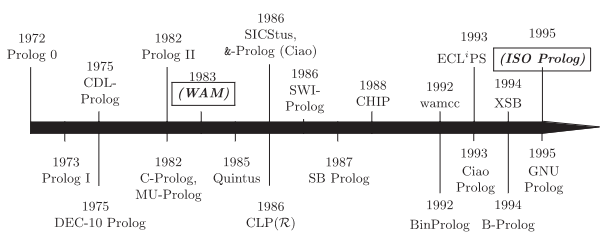
\includegraphics[scale=0.5]{images/prologhist.png}
    \caption{Evoluzione di Prolog \cite{korner2022fifty}}
    \label{fig:prologhist}
\end{figure}

Di seguito vedremo una panoramica delle principali tappe che hanno contrassegnato l'evoluzione di Prolog (vedi figura \ref{fig:prologhist}). Esploreremo le innovazioni chiave e i contributi accademici
che hanno, negli anni, arricchito il linguaggio. Vedremo poi le varie varianti di Prolog che sono state sviluppate nel corso degli anni, e come esse abbiano influenzato
il linguaggio principale.

Prolog fa parte principalmente di tre rami della ricerca: intelligenza artificiale, risoluzione automatica dei teoremi e processamento del linguaggio.

Il campo dell'intelligenza artificiale naque all'incirca nel 1956 e diede velocemente vita al linguaggio di programmazione funzionale LISP. Da li in poi 
l'interesse aumentò e diede vita ad altri linguaggi più o meno ad alto livello.

La soluzione automatica di teoremi è un campo della matematica che si occupa di trovare dimostrazioni automatiche di teoremi matematici. La risoluzione può essere utilizzata per ottenere una procedura semi-decisionale per la logica predicativa ed è al centro della maggior parte delle procedure di inferenza nella programmazione logica.

A seguito di questi progressi, un visionario precoce nello sviluppo del campo della programmazione logica è stato Cordall Green, che già alla fine degli anni 60 immaginava come estendere la risoluzione per costruire 
automaticamente la soluzione di un problema. In particolare voleva applicare questo strumento per la risoluzione di domande basate sulla logica di primordine. Questo rappresentò il primo zenit della programmazione logica impiegata in applicazioni di AI.

Un altro progetto notabile è quello di Ted Elcock che sviluppò Absys, un linguaggio di programmazione dichiarativo che anticipò alcune delle funzioni di Prolog come la negazione come fallimento, operatori di aggregazione e il backtracking.

Nel frattempo Alain Colmerauer stava provando a sviluppare un sistema di conversazione uomo-macchina, ciò lo portò a sviluppare Q-systems, un sistema impegato per le traduzioni da Inglese a Francese dei rapporti meteorologici Canadesi. 
Il suo obiettivo di modificare Q-systems, per ottenere un sistema domanda e risposta, lo portò a sviluppare un linguaggio di programmazione basato sulla logica predicativa. Questo linguaggio fu chiamato Prolog, e fu sviluppato nel 1972.
Il suo creatore, Alain Colmerauer, diede quindi vita a Prolog nel 1972. Il risultato fu non solo la prima applicazione del linguaggio naturale (NL) di quello che oggi conosciamo come Prolog, ma la base di Prolog stesso: un sistema di risoluzione
lineare ristretto alle clausole di Horn che poteva risolvere problemi in maniera non deterministica.

L'articolo di K{\"o}rner \cite{korner2022fifty} fornisce una panoramica completa dell'evoluzione di Prolog, e di come questo linguaggio sia stato influenzato nel corso degli anni. Io mi concentrerò soltato su alcuni aspetti chiave che hanno portato Prolog a diventare il linguaggio che conosciamo oggi.
Se siete interessati a una panoramica più completa seguendo una linea temporale come quella in figura \ref{fig:prologhist} vi consiglio caldamente di leggere l'articolo.
\subsection{Tappe fondamentali dell'evoluzione di Prolog}
\label{subsec:tappe}
Nella sua prima decade di vita Prolog subì molte variazioni, la sua prima versione fu Prolog 0, seguita da Prolog 1. In queste versioni il linguaggio
prevedeva già qualche predicato built in che poi fu incluso nello standard ISO. Queste versioni includevano già il predicato \verb+dif/2+, questo predicato fu importante perchè fece prendere piede al concetto di unificazione. Successivamente seguì l'aggiunta
della negazione come fallimento, questa fu una delle aggiunte più importanti, in quanto permise di risolvere problemi che non erano risolvibili con la sola unificazione.

Nel 1974 David H.D. Warren sviluppò Warplan, un sistema di pianificazione automatica basato su Prolog. Lo sviluppo di questo progetto, che poi divento la sua tesi di dottorato, lo portò a voler ottimizzare l'interprete Prolog, siccome ritenuto lento rispetto ad altri linguaggi di più alto livello come LISP.
Sviluppò quindi un nuovo interprete, chiamato WAM (Warren Abstract Machine).

\begin{figure}[h!]
    \centering
    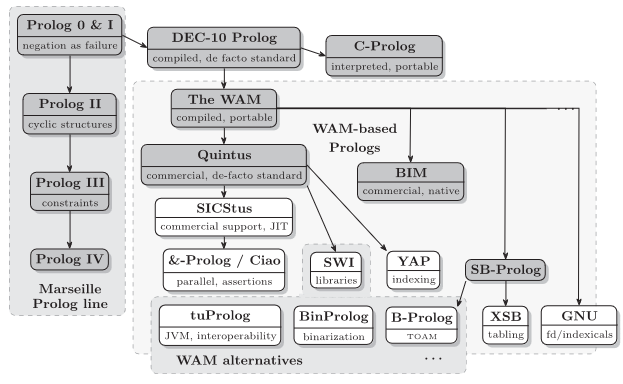
\includegraphics[scale=0.55]{images/prologimpl.png}
    \caption{Quandro generale delle versioni di Prolog \cite{korner2022fifty}}. In grigio scuro sono riportate le versioni che ad oggi (2022 \cite{korner2022fifty}) non sono più supportate.
    \label{fig:prologimpl}
\end{figure}

WAM era, ed è tutt'ora, lo standard per i compilatori Prolog. Due delle implemenatazioni più di successo 
sono \textit{GNU Prolog} e quella utilizzata per il mio progetto \textit{SWI-Prolog}. Entrambe queste implementazioni sono open source e disponibili online.

GNU Prolog è un compilatore Prolog gratuito e open source, è stato sviluppato da Daniel Diaz. È stato sviluppato per essere un compilatore Prolog standard, e quindi non include estensioni proprietarie. La sua implementazione utilizza WAM come base per produrre codice in C che verrà poi compilato da GCC. C fu poi rimpiazzato da un linguaggio miniassembly specializzato
perchè ritenuto più efficiente. 

SWI-Prolog naque dalla mancanza di Quintus (un implementazione di Prolog) di chiamate ricorsive tra Prolog e C. La potenza di questa implementazione è la community che la supporta, infatti è una delle implementazioni più utilizzate al mondo sia per la ricerca che non. Oltre che la forte community
SWI-Prolog, al contrario di GNU Prolog, è interpretato, e non compilato. Questo permette di avere un ambiente di sviluppo molto più flessibile e adatto alla ricerca.

Questo, come detto in introduzione, è solo un breve riassunto delle tappe fondamentali dell'evoluzione di Prolog. Se siete interessati a una panoramica più completa vi consiglio caldamente di leggere l'articolo di K{\"o}rner \cite{korner2022fifty}. 
Nell'articolo viene descritto in modo più dettagliato ISO Prolog e le differenze tra le varie versioni utilizzate al giorno d'oggi.
\section{Lavori notabili}
\label{sec:lavori}
Lo scopo di questa sezione è di presentare i lavori più notabili che hanno utilizzato Prolog o comunque un linguaggio logico per risolvere problemi di task planning e intelligenza artificiale.
Durante lo sviluppo del progetto è stato necessario avere dei lavori di riferimento per poterlo poi sviluppare in modo corretto.
Premesso questo non voglio quindi entrare troppo in dettaglio, ma soltanto illustrare i lavori lasciando al lettore la possibilità di approfondirli.

Un lavoro che mostra come i linguaggi di programmazione logica, e in particolare Prolog, possano essere usati per risolvere problemi di task planning è sicuramente quello di Meli \cite{meli2023logic}. In questo lavoro viene presentato lo stato dell'arte del task planning, e come questo possa essere risolto con un linguaggio di programmazione logica.
L'articolo inizia introducendo la necessità del mondo di oggi di progettare sistemi robotici con capacità di decisione deliberativa. 
Continua poi spiegando i requisiti per un sistema robotico deliberativo, quelli identificati sono questi moduli (vedi figura \ref{fig:delrob}): 
    \textit{planning},
    \textit{acting},
    \textit{monitoring},
    \textit{observing},
    \textit{goal reasoning},
    \textit{learning}.
\begin{figure}[h!]
    \centering
    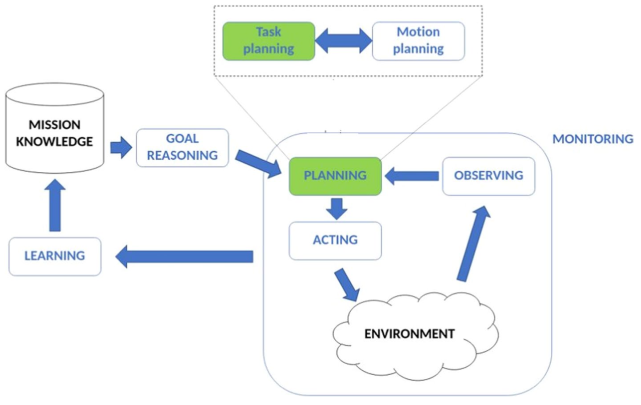
\includegraphics[scale=0.55]{images/deliberativerobot.png}
    \caption{Funzioni di un robot deliberativo \cite{meli2023logic}}
    \label{fig:delrob}
\end{figure}
Un sistema robotico è quindi un gruppo di robot con un obiettivo comune, questo può essere portato a termine attraverso un insieme di azioni che possono essere compiute dal robot nel mondo.
Il paper poi continua introducedo la tassonomia dei task planner e poi introduce i tre tipi di logica identificati per creare un task planner: \textit{logica standard}, \textit{logica temporale} e \textit{logica probabilistica}.
Da qui il paper introduce la task usata come esempio: \textit{Peg transfer task}, in italiano compito di trasferimento perni.
Il compito consiste nel posizionare gli elastici di un determinato colore nel perno del colore corrispondente.
Viene poi formalizzata in \textit{PDDL}, un linguaggio di descrizione di domini di pianificazione. Questo è stato fatto con l'obiettivo, poi, di tradurlo in un linguaggio logico.
Segue poi una descrizione della soluzione del problema nei tre tipi di logica precedentemente descritti. Conclude poi con una discussione dei risultati ottenuti spieganfo come la logica standard sia la più adatta per risolvere questo tipo di problemi.

Un altro lavoro che utilizzò Prolog fu \textit{Fifth Generation Computer Systems}. Questa fu una iniziativa di 10 anni, promossa dal Giappone, che aveva come obiettivo quello di creare i computer utilizzando tanta programmazione logica e programmazione parallela.
Questo perchè come obiettivo finale si volevano avere dei sistemi per la ricerca in ambito di intelligenza artificiale. Più informazioni a riguardo di questo progetto possono essere trovate nel lavoro di K\"orner \cite{korner2022fifty}.

Anche la nota azienda IBM utilizzò Prolog per lo sviluppo di un computer capace di rispondere alle domande. Questo fu sviluppato nel 2011 e prese il nome di \textit{Watson}. Nel 2013 IBM annuciò che Watson sarebbe stato utilizzato per l'aiuto a prendere decisioni riguardo al trattamento del cancro ai polmoni. Prolog è stato usato per creare la base di conoscenza e per l'analisi del linguaggio.
Una curiosità è che anche la nostra università ha partecipato allo sviluppo iniziale di Watson insieme ad altre università statunitensi. %come cito?.

Un ultimo lavoro che utilizza Prolog per il design di un braccio robotico è \textit{Design an Arm Robot through Prolog Programming Language} \cite{mustafa2013design}. Lo scopo di questo articolo era quello di progettare un braccio robotico comandato da un programma Prolog. Nel paper viene introdotto il caso di studio fornendo al lettore le nozioni base di robot e sistema intelligente.
Nella seconda parte poi viene spiegato il design utilizzato per il sistema Prolog e come è stato implementato, includendo anche il codice.

Questi sono alcuni dei lavori più interessanti che ho trovato sia per il campo della robotica che per quello dell'intelligenza artificiale. Prolog ha una storia che conta più di 50 anni e quindi è stato utilizzato in molti altri lavori. Questa panoramica serviva per capire le potenzialità di Prolog
e come questo sia utilizzato al giorno d'oggi. La ricerca nell'ambito di Prolog e dell'intelligenza artificiale continua a progredire, portando ad importanti sviluppi. Oltre al campo della robotica e dell'intelligenza artificiale, è rilevante menzionare anche l'intelligenza artificiale neurosimbolica. Questo approccio combina elementi di intelligenza artificiale simbolica, come Prolog, con tecniche di intelligenza artificiale ispirate al funzionamento del cervello, come le reti neurali artificiali. L'integrazione di questi due paradigmi promette di aprire nuove strade nel campo dell'intelligenza artificiale e potenzialmente superare alcune delle limitazioni dei singoli approcci. La ricerca in questo ambito è in continua evoluzione, offrendo nuove prospettive e sfide interessanti.

%TODO  RILEGGERE INTERAMENTE, PRIMA PARTE DA RIVEDERE. NON MI PIACE TROPPO LA FORMA DELLA PRIMA SECTION
%TODO  RILEGGERE TUTTO IL DOCUMENTO E CORREGGERE GLI ERRORI DI GRAMMATICA E SINTASSI
%TODO  VEDERE SE PARTE STORIA E LAVORI NOTABILI HA FILO E SENSO.
